\chapter{Xây dựng hệ thống gợi ý sản phẩm dựa trên mô hình ``Auto-Encoder''}
\graphicspath{{Chapter3/Chapter3Figs}}
\label{Chapter3}

\textit{Chương này trình bày về cách áp dụng mô hình "Variational Auto-Encoder" để giải quyết bài toán xây dựng hệ thống gợi ý sản phẩm \cite{mvae}; đây là cách giải quyết bài toán mà chúng tôi tập trung tìm hiểu trong khóa luận. 
Đầu tiên, chúng tôi phân tích hai loại dữ liệu phản hồi được dùng trong bài toán này từ người dùng là:
``explicit feedback'' và ``implicit feedback'' và lý do chúng tôi đặc biệt quan tâm xây dựng hệ thống gợi ý với dữ liệu ``implicit feedback''.
Sau đó, chúng tôi trình bày về cách áp dụng mô hình ``Auto-Encoder'' để có thể xây dựng được một hệ thống gợi ý sản phẩm ở mức cơ bản. 
Cuối cùng, chúng tôi trình bày các phần tinh chỉnh để có được một mô hình gợi ý sản phẩm tốt hơn, bao gồm: áp dụng kỹ thuật ``drop-out'' khi huấn luyện mô hình, thay mô hình ``Auto-Encoder'' bằng một biến thể của nó là ``Variational Auto-Encoder'' và thay đổi hàm mục tiêu để phù hợp hơn với bài toán xây dựng hệ thống gợi ý.}


\section{Dữ liệu phản hồi của người dùng trong bài toán xây dựng hệ thống gợi ý sản phẩm}
    Như đã trình bày ở phần~\ref{Chapter1}, để xây dựng một hệ thống gợi ý 
    theo hướng tiếp cận ``Collaborative filtering'' ta chỉ cần dữ liệu là ma trận tương tác của người dùng.
    Tương tác ở đây có nghĩa là các phản hồi của người dùng dành cho sản phẩm, và các phản hồi này bao gồm hai loại:
    \begin{itemize}
        \item Phản hồi cụ thể ``explicit feedback''
        \item Phản hồi ngầm ``implicit feedback''
    \end{itemize}
    Trong phần này, chúng tôi sẽ làm rõ về tính chất của hai loại dữ liệu phản hồi cũng như ảnh hưởng của chúng đến hệ thống gợi ý.
    \subsection{Dữ liệu ``explicit feedback''}
    Dữ liệu ``explicit feedback'' được hiểu là những
    phản hồi của khách hàng về sản phẩm một cách tường minh và cụ thể, ví dụ như: số điểm đánh giá,
    bình luận, ... ``Explicit feedback'' có thể thể hiện rõ về mức độ thích/không thích của người dùng về sản phẩm;
    ví dụ người dùng có thể thể hiện sự yêu thích của họ từ 1 đến 5 sao cho một sản phẩm (một cách đánh giá thông dụng), 
    sản phẩm được đánh giá 5 sao chứng tỏ nó được thích hơn so với sản phẩm được đánh giá 4 sao. 
    Trong thực tế, dữ liệu ``explicit feedback'' thường khó để thu thập cũng như gặp trở ngại về tính tin cậy.
    Thu thập loại dữ liệu này gặp khó khăn vì không phải người dùng nào cũng sẵn sàng phản hồi về sản phẩm. 
    Sự miễn cưỡng của người dùng cũng như những tác động khi họ phản hồi có thể dẫn đến sự thiếu khách quan,
    làm sai lệch kết quả của hệ thống gợi ý. 
    Thêm nữa, vì phản hồi của người dùng thể hiện mức độ thích/không thích của người dùng, mà người dùng thì chỉ tương tác với
    một lượng sản phẩm nhỏ trên toàn hệ thống, những sản phẩm còn lại sẽ rơi vào trường hợp thiếu dữ liệu (``missing data''),
    gây khó khăn cho việc xử lí. 
    Ngày nay, số lượng sản phẩm trong hệ thống là rất lớn, ``explicit feedback'' sẽ gặp khó khăn rất lớn khi có quá nhiều trường hợp thiếu dữ liệu,
    tác động đáng kể đến hiệu quả của hệ thống. Mặt khác, ``collaborative filtering'' sẽ có cơ sở đánh giá nhóm người dùng ``tương đồng'' với nhau
    một cách khắt khe hơn, giúp các gợi ý là những sản phẩm ``tốt'' hơn, tuy nhiên đôi lúc làm cho các gợi ý không được đa dạng.

    \subsection{Dữ liệu ``implicit feedback''}
    Dữ liệu ``implicit feedback'' là dữ liệu được suy ra từ hành động của người dùng, nếu họ xem một bộ phim thì ta có thể hiểu là họ ``thích'' bộ phim đó. ``Implicit feedback'' cũng có thể được suy ra từ ``tín hiệu ngầm'' (``implicit signal''),
    xét ví dụ người dùng đánh giá một sản phẩm là 4 sao (trên thang đánh giá từ 1 đến 5 sao), từ ``tín hiệu ngầm'' dựa trên số sao họ đánh giá,
    ta có thể suy ra họ ``thích'' sản phẩm đó. 
    ``Implicit feedback'' chỉ thể hiện rõ về sự ``thích'' cũng như chỉ thể hiện một cách tương đối mức độ yêu thích của người dùng.
    Cụ thể, người dùng không xem một bộ phim không có nghĩa là họ không thích bộ phim đó, có thể là họ chưa xem hoặc không biết nó có trên hệ thống.
    Cũng như họ xem một bài hát 10 lần chứng tỏ họ thích hơn so với một bài hát họ chỉ nghe 2 lần, 
    và ``implicit feedback'' không thể thể hiện được rõ điều này.
    Trong thực tế, lượng dữ liệu phản hồi ngầm rất lớn và dễ dàng thu thập được, quá trình ``phản hồi'' của người dùng là bị động
    nên không bị ảnh hưởng bởi các yếu tố ngoại cảnh khác. 

    Ma trận tương tác của người dùng với dữ liệu phản hồi ngầm sẽ có dạng là một ma trận nhị phân, với giá trị \textbf{1} 
    thể hiện người dùng ``thích'' sản phẩm đó, giá trị \textbf{0} thể hiện hệ thống chưa có cơ sở để xác định người dùng ``thích'' sản phẩm đó.

    Với dữ liệu phản hồi ẩn, ``collaborative filtering'' sẽ xác định nhóm người dùng ``tương đồng'' với nhau rộng hơn
    do chỉ quan tâm đến các sản phẩm họ thích. Điều này sẽ giúp các gợi ý của hệ thống 
    đa dạng hơn, tuy nhiên các sản phẩm mà người dùng không thích cũng có thể sẽ được gợi ý.

    Trong giới hạn của khóa luận này, chúng tôi chỉ tìm hiểu về một hệ thống gợi ý với dữ liệu phản hồi ngầm do tính khách quan
    cũng như giải quyết được các khó khăn của ``explicit feedback''.

% \section{``Multinomial log-likelihood'' cho bài toán xây dựng hệ thống gợi ý}
\section{Áp dụng mô hình ``Auto-Encoder'' để xây dựng hệ thống gợi ý sản phẩm ở mức cơ bản}
    Như đã trình bày ở chương~\ref{Chapter2}, mô hình ``Auto-Encoder'' là một mạng nơ-ron thường được sử dụng trong tác vụ trích xuất đặc trưng ẩn thông qua phương pháp học không giám sát.
    Ở phần này, chúng tôi sẽ trình bày việc xây dựng một hệ thống gợi ý sản phẩm cơ bản dựa trên mô hình ``Auto-Encoder''.

    \subsection{Kiến trúc mô hình}
    \label{chap3/sec11}
    Phương pháp xây dựng mô hình gợi ý sản phẩm mà chúng tôi tìm hiểu đó là sử dụng kiến trúc ``Auto-Encoder'', một mạng nơ ron-nhận input đầu vào là một phần tương tác của người dùng trong quá khứ và mô hình được huấn luyện để tái tạo lại toàn bộ tương tác của người dùng. 
    Mô hình sẽ đưa ra gợi ý các tương tác cho người dùng dựa trên những tương tác được tái tạo lại.
    Mô hình này là một mạng nơ-ron bao gồm hai thành phần:
    \begin{itemize}
        \item Mạng nơ-ron ``encoder'' có chức năng rút trích đặc trưng ẩn từ những tương tác của người dùng trong lịch sử.
        \item Mạng nơ-ron ``decoder'' có chức năng tái tạo lại tương tác của người dùng từ đặc trưng ẩn.
    \end{itemize}

    % Mặc dù cách hoạt động của mô hình trong giai đoạn huấn luyện và trong giai đoạn kiểm tra có phần khác nhau, nhưng ở phần này chúng tôi chỉ trình bày cách hoạt động của mô hình trong giai đoạn huấn luyện để qua đó diễn giải kiến trúc mô hình một cách thuận tiện. Và sau đó chúng tôi sẽ trình bày cách để đưa ra gợi ý cho người dùng mới sau.


   Tập dữ liệu được sử dụng để huấn luyện bao gồm $U$ người dùng $\mathcal{U} = [u_1,u_2, .., u_U]$ và mục tiêu là xây dựng mô hình đưa ra gợi ý trên tập $I$ sản phẩm $\mathcal{I} = [i_1,i_2, ..., i_I]$. 
    Bên cạnh đó, dữ liệu tương tác của các người dùng với các sản phẩm sẽ được thể hiện bởi một ma trận tương tác $X \in \mathbb{N}^{U\times I}$. 
    Tương tác của một người dùng sẽ là một véc-tơ $x_u = [x_{u1}, x_{u2}, ..., x_{uI}] \in \mathbb{N}^I $ với $u \in \mathcal{U}$.
    
    Với giả định rằng mỗi người dùng sẽ có tồn tại một đặc trưng ẩn nào đó, đặc trưng ẩn này là yếu tố sẽ quyết định đến việc tương tác của người dùng lên các sản phẩm.
    Do đó, bằng cách dựa vào lịch sử tương tác của người dùng ta sẽ cố gắng để có thể trích xuất được đặc trưng ẩn của họ.
    Mô hình sẽ nhận đầu vào $x_u$ là dữ liệu tương tác của người dùng $u$, sau đó qua mạng encoder ta có được đặc trưng ẩn $z_u$.
    Từ đặc trưng ẩn $z_u$ có được, mạng decoder sẽ cố gắng tái tạo lại dữ liệu tương tác ban đầu.
    Điều đó sẽ giúp ta có được một đặc trưng ẩn thể hiện được những yếu tố quyết định đến tương tác của người dùng.
    Hay nói cách khác, ta hy vọng đặc trưng ẩn được trích xuất sẽ thể hiện cho sở thích của người dùng. 

    ``Auto-Encoder'' là một mạng nơ-ron thường được sử dụng để trích xuất đặc trưng ẩn bằng phương pháp học không giám sát.
    Một cách đơn giản để huấn luyện mô hình ``Auto-Encoder'' cho bài toán xây dựng hệ thống gợi ý là ta sẽ cố gắng tái tạo lại tương tác của người dùng.
    Dựa vào kết quả tương tác được tái tạo để gợi ý tập sản phẩm ``tốt'' nhất mà người dùng chưa tương tác trước đó. 
    Hoặc ta có thể xem như là một bài toán hồi quy, khi mà dữ liệu đầu vào là một con số thể hiện cho tương tác của người dùng.
    Kết quả của mô hình cũng là một véc tơ số ``gần'' với dữ liệu tương tác ban đầu.  
    Để áp dụng hướng tiếp cận cơ bản này, chúng tôi sẽ trình bày về kiến trúc của một mô hình Auto-Encoder để xây dựng hệ thống gợi ý cơ bản.
    \begin{figure}
        \centering
        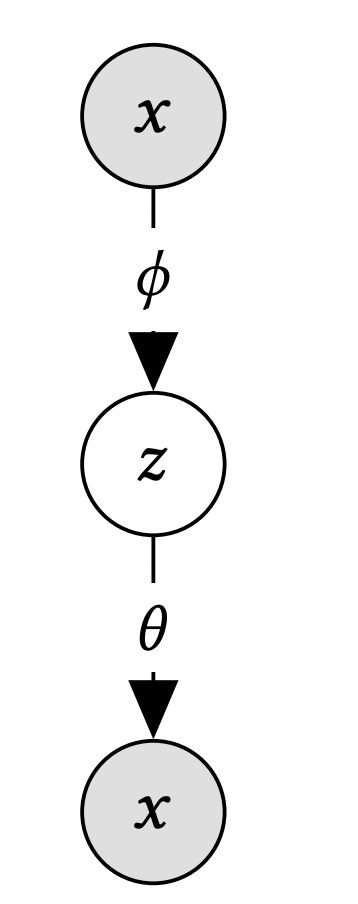
\includegraphics[width=0.2\textwidth]{ae.png}
        \caption{Minh họa kiến trúc mô hình Auto-Encoder cho bài toán gợi ý sản phẩm}
        \label{fig_recae}
    \end{figure}

    Mô hình được cấu thành từ hai mạng nơ-ron tách biệt được gọi là encoder và decoder. 
    Ta có thể xem rằng mạng nơ-ron encoder là một hàm phi tuyến ánh xạ dữ liệu đầu vào ở chiều không gian cao, $x_u \in R^I$ sang một không gian thấp hơn để biểu diễn cho đặc trưng ẩn $z_u \in R^k$ với $k$ là số chiều của không gian đặc trưng ẩn. 
    Thường thì $k$ sẽ rất nhỏ so với $I$. Cụ thể thì ta có:
    \begin{equation}
        z_u = g_\phi(x_u) = g(W^T x_u + b_1)
    \end{equation}

  
    trong đó $g(.)$ là hàm kích hoạt phi tuyến và $\phi = (W,b_1)$, với $W\in R^{I\times k}$, $b_1 \in R^{k}$ tương ứng sẽ là trọng số và hệ số ``bias'' của mạng nơ-ron encoder. 

    Sau khi có được đặc trưng ẩn, $z_u$ sẽ được truyền thẳng qua mạng nơ-ron decoder nhằm mục đích xây dựng lại tương tác ban đầu từ $z_u$
    \begin{equation}
        \widehat{x}_u = f_\theta(z_u) = f(V^T z_u + b_2)
    \end{equation}

    Tương tự với encoder, $\theta = (V,b_2)$, với $V\in R^{k\times I}$, $b_2 \in R^{k}$  sẽ tương ứng là các trọng số và ``bias'' của mạng nơ ron và $f(.)$ chính là hàm kích hoạt phi tuyến của mạng nơ-ron.
    Hình \ref{fig_recae} minh họa cho kiến trúc Auto-Encoder cho bài toán gợi ý sản phẩm

    \subsection{Quá trình huấn luyện và đưa ra gợi ý}
    
    Để huấn luyện một mô hình ``Auto-Encoder'' cho bài toán xây dựng gợi ý sản phẩm, ta cần cực tiểu hóa hàm lỗi giữa tương tác được mô hình tái tạo lại và dữ liệu tương tác đầu vào sau:
    \begin{equation}
        \label{ae_rec_loss}
        \mathcal{L}(x;\phi,\theta) = \frac {1}{U}\sum_{x_u \in X}(||x_u - h_{\phi,\theta}(x_u)||^2_2)
    \end{equation}
    trong đó $h_{\phi,\theta}(x_u)$ là tương tác được tái tạo lại với dữ liệu đầu vào là tương tác của người dùng ban đầu $u \in \mathcal{U}$ và $x_u \in R^I$.
    \begin{equation}
        h(x_u;\theta) = f(V^T z_u+ b_2) = f(V^T g(W^T x_u + b_1) + b_2)
    \end{equation}    
    với $f(.)$ và $g(.)$ sẽ là các hàm kích hoạt phi tuyến của mạng nơ-ron.
    
    Với hàm lỗi \ref{ae_rec_loss} mô hình hy vọng sẽ có thể tự động trích xuất được những đặc trưng ẩn có thể được dùng để hình thành nên các tương tác của người dùng.
    Mô hình sẽ được huấn luyện và tìm ra bộ tham số $\theta^*$ sao cho tối thiểu được độ lỗi \ref{ae_rec_loss}: 
    \begin{equation}
        \theta^* = \text{arg}_\theta \text{min}  \mathcal{L}(x;\theta)
    \end{equation}    
    

    Tuy nhiên, để tránh tình trạng ``overfitting'' sẽ thường xảy ra khi huấn luyện một mạng nơ-ron phi tuyến, gây ảnh hưởng đến độ chính xác của mô hình. 
    Chúng ta cần phải thêm một lượng ``regularization'' cho bộ tham số $(\phi,\theta)$.
    ``Regularization'' nói một cách đơn giản là thay đổi mô hình một chút để tránh ``overfitting'' trong khi vẫn giữ được tính tổng quát của nó (tính tổng quát là tính mô tả được nhiều dữ liệu, trong cả tập dữ liệu huấn luyện và dữ liệu kiểm định).
    Cụ thể chúng tôi dùng ``L2 regularization'' cho mô hình.
    Vậy nên để huấn luyện mô hình ``Auto-Encoder'' với bài toán xây dựng hệ thống gợi ý sản phẩm ta sẽ huấn luyện mô hình để tìm được bộ tham số cho mô hình  như sau:
    \begin{equation}
        \label{ae_rec_obj}
        \theta^* = \text{arg}_\theta \text{min}  \mathcal{L}(x;\theta)  + \frac \lambda 2 \times (||W||^2_2 + ||V||2_2)
    \end{equation}
    trong đó $\lambda$ là hệ số ``regularization''.

    Với kiến trúc trên, mô hình xây dựng cho hệ thống gợi ý với số lượng sản phẩm là I và đặc trưng ẩn với số chiều là k thì số lượng tham số của mô hình sẽ là $2Ik + I + k$.
    
    Sau khi huấn luyện mô hình với hàm mục tiêu trên, ta tìm được được bô tham số $\theta^*$, thì để dự đoán tương tác của người dùng u với sản phẩm i cụ thể sẽ là: 
    $$\widehat{x}_{ui} = h(x_{ui},\theta^*)$$
    Với tương tác được dự đoán, cụ thể là những tương tác lên những sản phẩm chưa được người dùng thực hiện trước đó, ta chọn ra những sản phẩm có kết quả trả về cao nhất để có thể đưa ra gợi ý cho người dùng. 


    \subsection{Thay đổi ``input'' và ``output'' trong quá trình huấn luyện mô hình để phù hợp hơn với bài toán gợi ý sản phẩm}
    \label{DAE_recsys}
    \begin{figure}
        \centering
        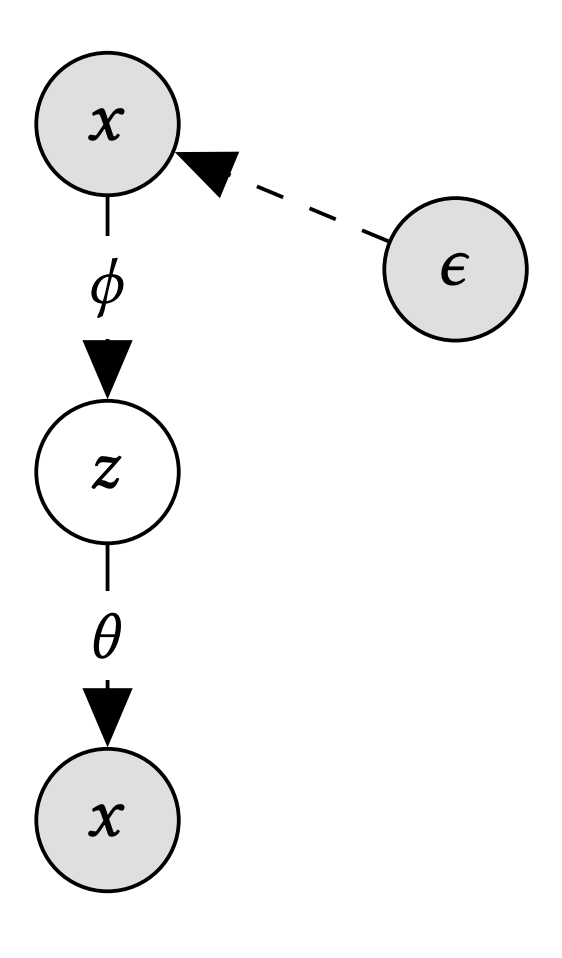
\includegraphics[width=0.3\textwidth]{dae.png}
        \caption{Minh họa kiến trúc mô hình ``Denoising Auto-Encoder'' cho bài toán gợi ý sản phẩm}
        \label{fig_recdae}
    \end{figure}
    Như đã thảo luận ở phần \ref{chap3/sec11} trên, chúng ta đã xây dựng một kiến trúc ở mức cơ bản nhất trong việc xây dựng một hệ thống gợi ý sản phẩm dựa trên mô hình ``Auto-Encoder''.
    Tuy nhiên, mô hình trên vẫn còn nhiều hạn chế: 
    \begin{itemize}
        \item Thực tế thì mô hình vẫn đang làm tác vụ là tái tạo lại tương tác của người dùng chứ chưa thực sự được huấn luyện để dự đoán những sản phẩm mà người dùng sẽ tương tác dựa lịch sử tương tác của họ.
        \item Một hạn chế khác đó là tình trạng ``overfiting'', khi huấn luyện mạng nơ-ron. Với việc thêm hệ số ``regularization'' để huấn luyện nhưng với dữ liệu thưa thì việc chính quy hóa sẽ không thực sự hiệu quả. 
    \end{itemize}
    
    Một phương pháp mà chúng tôi sử dụng để có thể giải quyết những vấn đề trên đó là chúng tôi ``che'' đi một số tương tác trước khi dữ liệu được truyền thẳng qua mạng encoder. 
    Nói cách khác là chúng tôi áp dụng kỹ thuật ``dropout'' cho véc-tơ đầu vào, ``dropout'' là một phương pháp ``regularization'' thường được áp dụng khi huấn luyện các mạng học nơ-ron \cite{Goodfellow-et-al-2016-Book}.
    ``Dropout'' huấn luyện một tập các mạng con mà các mạng con này được định nghĩa bằng cách bỏ đi một số nơ-ron (không phải nơ-ron đầu ra) của mạng ban đầu. 
    Trong thực tế, để bỏ đi một số nơ-ron ta chỉ nhân cho giá trị đầu ra của nó cho 0. 
    ``Dropout'' sẽ ép mạng nơ-ron tìm ra được những đặc trưng quan trọng hơn, hay là tìm ra những sản phẩm ảnh hưởng lớn đến đặc trưng ẩn của người dùng. 
    
    Mô hình ``Auto-Encoder'' với đầu vào được ``che'' đi trong quá trình huấn luyện là ``Denoising Auto-Encoder'' như đã trình bày trong phần~\ref{chap2/subsec12}.

    Gọi $\tilde{x}$ sẽ là dữ liệu sau khi đã ``che'' đi một số các tương tác, $\tilde{x}$ sẽ được truyền thẳng qua mạng encoder để trích xuất được đặc trưng ẩn:
    \begin{equation}
        \label{z_u_with_x_tilde}
        z_u = g(W^T \tilde{x}_u + b_1)
    \end{equation}
    
    Với việc sử dụng thêm ``nhiễu'' vào dữ liệu tương tác ban đầu của người dùng sẽ mang lại cho mô hình ``Auto-Encoder'' phù hợp hơn và hiệu quả hơn khi huấn luyện với dữ liệu tương tác của người dùng.
    Nói cách khác đó là sau khi thực hiện thêm nhiễu, mô hình sẽ thực sự là dự đoán những tương tác bị che từ những tương tác có trước đó trong lịch sử của người dùng thay vì chỉ để tái tạo lại tương tác của người dùng trước đó.

    Bên cạnh đó, ``dropout'' là một kỹ thuật khi huấn luyện mạng nơ-ron để ngăn tình trạng ``overfitting'' hiệu quả.
    Hình \ref{fig_recdae} thể hiện cho ý tưởng sử dụng kiến trúc denosing Auto-Encoder cho bài toán gợi ý sản phẩm.     

    

\section{Tinh chỉnh cách áp dụng mô hình ``Auto-Encoder'' để có được hệ thống gợi ý sản phẩm hoạt động tốt hơn}
    Trong lĩnh vực trí tuệ nhân tạo, dữ liệu đóng vài trò cực kỳ quan trọng.
    Đặc biệt là lĩnh vực máy học, việc hiểu được dữ liệu sẽ góp phần không nhỏ đến việc xây dựng một mô hình hiệu quả. 
    Đối với bài toán xây dựng hệ thống gợi ý sản phẩm, trong thực tế mỗi người dùng sẽ chỉ tương tác với một lượng nhỏ số lượng sản phẩm trên toàn bộ hệ thống.
    Điều này dẫn đến dữ liệu tương tác của người dùng sẽ là dữ liệu thưa.
    Với đặc điểm này, tác giả Liang trong bài báo \cite{mvae} mà chúng tôi tìm hiểu trong khóa luận đã đề xuất việc sử dụng mô hình ``Variational Auto-Encoder'' (VAE), một biến thể đặc biệt của ``Auto-Encoder'' cơ bản để xây dựng hệ thống gợi ý sản phẩm. 
    Bên cạnh đó, tác giả Liang cũng đã có một số tinh chỉnh về hàm chi phí giúp mô hình hoạt động tốt hơn.

    Trong phần này chúng tôi sẽ trình bày về kiến trúc mô hình VAE cũng như là những cải thiện cho mô hình trong tác vụ gợi ý sản phẩm cho người dùng được đề xuất trong bài báo \cite{mvae}. 

    \subsection{Thay ``Auto-Encoder'' bằng ``Variational Auto-Encoder''}
    
    Dữ liệu tương tác trong hệ thống gợi ý sản phẩm thường là dữ liệu thưa, có nghĩa là các phần tử trong véc-tơ input đầu vào sẽ đa phần sẽ mang giá trị 0. 
    Ngoài ra, mục tiêu của một hệ thống gợi ý sản phẩm chính là việc tăng thêm số lượng tương tác của người dùng lên hệ thống, đặc biệt là khi người dùng chưa tương tác nhiều.
    % Do đó, trong trường hợp này, nếu áp dụng những phương pháp dựa trên mạng nơ-ron thông thường sẽ dễ dẫn đến tình trạng ``overfitting'' khi mà dữ liệu đầu vào ít nên mô hình không học được.
    Do đó, trong trường hợp này nếu áp dụng các mô hình ``Auto-Encoder'' truyền thống sẽ dẫn đến tình trạng ``overfitting'', nghĩa là không sinh ra được gợi ý cho người dùng.
    
    Dựa vào hạn chế này, bài báo đã đề xuất việc sử dụng mô hình ``Variational Auto-Encoder''.
    Đây là một mô hình mạng nơ-ron nhưng với nền tảng xác suất, cụ thể là phương pháp Variational Inference - một phương pháp suy diễn dữ liệu trong lĩnh vực xác suất thống kê.
    Như đã trình bày ở phần~\ref{chap2/sec2}, đây là một biến thể đặc biệt của ``Auto-Encoder'' cơ bản, với việc đặc trưng ẩn được rút trích là một phân phối xác suất, mô hình đã mang lại ý nghĩa xác suất cho đặc trưng ẩn.
    Nói cách khác, đặc trưng giờ đây không chỉ thể hiện cho tương tác của người dùng, ngoài ra, là một phân phối xác suất thì đặc trưng ẩn còn có thể thể hiện được sự không chắc chắn ở trong đó, và sự không chắc chắn này có thể phần nào giúp giảm hiện tượng ``overfitting''.


    % Nếu ta sử dụng tất cả tương tác của người dùng để trích xuất được những đặc trưng ẩn, thì có thể sẽ bị ảnh hưởng bởi nhiễu, hay có thể sẽ có những sản phẩm ``không quan trọng'' trong việc thê hiện đặc trưng của người dùng nên đặc trưng ẩn sẽ mang theo tất cả các thông tin đó, điều này có thể dẫn đến việc overfiting khi dữ liệu thưa, hay tương tác của người dùng còn ít.
    % Những sản phẩm ``không quan trọng'' có thể xen là những sản phẩm mà không xuất hiện theo mẫu tương tác chung giữa các người dùng, những sản phẩm có thể sẽ là những sản phẩm đặc biệt của những người dùng có sở thích ``khác biệt'' so với những người dùng còn lại. 
    % Vì theo ý tưởng của collaborative, là hướng tiếp cận mà nhóm tìm hiểu để xây dựng hệ thống gợi ý, thì việc đưa ra gợi ý cho một người dùng sẽ dựa trên việc mô hình tìm ra được những mẫu tương tác chung giữa các người dùng và mẫu tương tác chung này sẽ được thể hiện thông qua đặc trưng ẩn.
    % Ngược lại, nếu từ tương tác của người, ta phát sinh một phân bố để thể hiện cho đặc trưng ẩn, thì khi sử dụng đặc trưng ẩn để đưa ra gợi ý, thì điểm ``tốt nhất'' trong phân bố, cụ thể ở bài báo được đề xuất là giá trị trung bình của phân bố sẽ được lấy để đưa ra gợi ý.
    % Vì là một phân bố, những sản phẩm ``ko quan trọng'' sẽ ít đóng góp ít hơn ở điểm trung bình. Vì điểm trung bình sẽ là điểm có phân phối xác suất cao nhất, có nghĩa là tập sản phẩm ít xuất hiện trong xu hướng tương tác chung của các người dùng trong hệ thống sẽ đóng góp ít hơn ở điểm trung bình.     

<<<<<<< HEAD
    \subsubsection{Kiến trúc mô hình}
    Để áp dụng variational Auto-Encoder cho việc xây dựng một hệ thống gợi ý sản phẩm, ta sẽ xét variational với 2 tiến trình riêng biệt. 
=======
    
    Để áp dụng ``Variational Auto-Encoder'' (VAE) cho việc xây dựng một hệ thống gợi ý sản phẩm, ta sẽ xét VAE với 2 tiến trình riêng biệt. 

>>>>>>> 1fb170123ba595a507b570a6bb9f69e8c4a0167d
    Đầu tiên là tiến trình suy diễn, tiến trình này suy diễn đặc trưng ẩn của dữ liệu từ tương tác của người dùng.
    Có nghĩa là tìm ra phân phối bố của đặc trưng ẩn dựa trên dữ liệu tương tác của người dùng. 
    Tiến trình này được thực hiện thông qua một mạng nơ-ron được gọi là encoder hay còn được gọi là mạng inference.
    
    Tiếp theo là tiến tình phát sinh, tiến trình này có mục tiêu là phát sinh tương tác của ngời dùng từ đặc trưng ẩn.
    Cụ thể, từ phân phối có được từ tiến trình suy diễn, một đặc trưng ẩn sẽ được lấy mẫu từ phân phối trên. 
    Đặc trưng ẩn này sẽ tiếp tục đường truyền thẳng thông qua một mạng nơ-ron được gọi là decoder hay còn được gọi là mạng generative.
    Kết quả trả về sẽ là 1 véc-tơ thể hiện cho tương tác của người dùng được phát sinh từ đặc trưng ẩn.


    Encoder được dùng để xấp sỉ được ``posterior'' $p(z_u|x_u)$ thông qua phương pháp Variational Inference. 
    Như đã trình bày ở phần \ref{chap2/subsec21}, phương pháp này xấp xỉ ``posterior'' thông qua một phân phối $q$ cùng ``họ'' phân phối và đơn giản hơn để tính toán.
    Giả định rằng $p(z_u) = \mathcal{N}(0,I)$ là một phân phối chuẩn, thể hiện phân phối xác suất trên không gian của đặc trưng ẩn.
    Do đó, $p(z_u|x_u)$ và $q(z_u|x_u)$ sẽ thuộc cùng họ phân phối ``Gaussian''. 
    Khi đó $q(z_u|x_u) = \mathcal{N}(\mu_u,\sigma_u^2)$, bằng cách tối thiểu $\mathbb{KL}(q(z_u||x_u) || p(z_u|x_u))$ tìm ra bộ tham số định nghĩa cho phân phối $q$ sao cho $q(z_u | x_u)$ xấp sỉ được $p(z_u|x_u)$.    

    Tuy nhiên với phương pháp này, thì số lượng tham số sẽ tỉ lệ với số lượng người dùng và số lượng sản phẩm.
    Với số lượng tham số như vậy thì nó có thể sẽ dẫn đến các khó khăn khi xây dựng hệ thống gợi ý sản phẩm.
    Do đó ta sẽ sử dụng phương pháp ``amortized inference'', phương pháp này thay vì ta tìm trọng số mỗi người dùng độc lập với nhau thì các người dùng sẽ được chia sẻ chung bộ trọng số.
    Có nghĩa là phân phối đặc trưng ẩn của toàn bộ người dùng, $\mu_u \in R^k $ và $\sigma_u \in R^k $ sẽ được định nghĩa bởi mạng nơ-ron:
    \begin{equation}
        [\mu_u,\sigma_u] = g(x_u;\phi) \in R^{2k}
    \end{equation}
    với $k$ là số chiều của đặc trưng ẩn, $[.]$ là phép nối 2 véc-tơ, $f(.)$ sẽ là mạng nơ-ron với hàm kích hoạt phi tuyến với bộ trọng số $\phi$ được học qua quá trình lan truyền ngược.
    Lúc này, encoder sẽ là một mạng nơ-ron định nghĩa cho phân phối:
    \begin{equation}
        \label{inference_net}
        q_\phi(z_u|x_u) = \mathcal{N}(\mu_\phi(x_u),\sigma^2_\phi(x_u))
    \end{equation}
    

<<<<<<< HEAD
    Với $x_u$ là dữ liệu tương tác của người dùng, tương tự như kiến trúc mô hình đã được tình bày trước đó ở mục \ref{chap3/sec11}.
    Trước khi dữ liệu được truyền thẳng qua mạng encoder thì $x_u$ sẽ được thêm nhiễu thông qua một tầng drop-out. 
    Sau khi drop-out ta có được $\tilde{x}_u$. 
    Lúc này $\tilde{x}_u$ sẽ được truyền qua mạng encoder. 
=======
    Với $x_u$ là dữ liệu tương tác của người dùng, tương tự như kiến trúc mô hình đã được tình bày trước đó.
    Trước khi dữ liệu được truyền thẳng qua mạng encoder thì $x_u$ sẽ được thêm nhiễu thông qua một tầng ``drop-out''. 
    Sau khi drop-out ta có được $\tilde{x}_u$. 
    Lúc này $\tilde{x_u}$ sẽ được truyền qua mạng encoder. 
>>>>>>> 1fb170123ba595a507b570a6bb9f69e8c4a0167d
    Sau khi $\tilde{x}_u$ được truyền qua mạng encoder \ref{inference_net}, thì ta có được $z_u$.
    \begin{equation}
        \label{sampling_zu}
        z_u \sim q_\phi(z_u|\tilde{x}_u)
    \end{equation}
<<<<<<< HEAD
    Tương tự với Auto-Encoder thì $z_u$ sẽ được truyền thẳng qua một mạng nơ-ron phi tuyến. 
    Như đã trình bày ở phần \ref{chap2/subsec21} thì mô hình decoder sẽ định nghĩa cho likelihood của mô hình, có nghĩa là:
=======
    Tương tự với ``Auto-Encoder'' thì $z_u$ sẽ được truyền thẳng qua một mạng nơ-ron phi tuyến là decoder. 
    Như đã trình bày ở phần trên thì mô hình decoder sẽ định nghĩa cho likelihood của mô hình, có nghĩa là:
>>>>>>> 1fb170123ba595a507b570a6bb9f69e8c4a0167d
    \begin{equation}
        \label{generative_net}
        p_\theta(x_u|z_u) = f(z_u;\theta)
    \end{equation}

    Kết hợp encoder \ref{inference_net} và decoder \ref{generative_net} lại ta sẽ có một kiến trúc cơ bản của mô hình ``Variational Auto-Encoder'' cho bài toán xây dựng hệ thống gợi ý sản phẩm.

    \subsubsection{Quá trình huấn luyện}
    Để huấn luyện một mô hình Variational Auto-Encoder thì ta sẽ có hàm mục tiêu là hàm evidence lower bound (ELBO) như sau:
    \begin{equation}
        \label{elbo_mvae}
        \mathcal{L}(x_u;\phi,\theta) = E_{q_\phi(z_u|x_u)}[\log p_\theta(x_u|z_u)] - \mathbb{KL}(q_\phi(z_u|x_u) || p(z_u))
    \end{equation}
    trong đó $p_\theta(x_u|z_u)$ được thể hiện bởi một mạng nơ ron, qua công thức \ref{generative_net} và $q_\phi(z_u|x_u)$ là một mạng nơ-ron, được thể hiện ở công thức \ref{inference_net}.

    Để tìm được $\phi$ và $\theta$ ta sẽ thực hiện cực đại hóa, hay tối thiểu hóa giá trị âm của ELBO, sau đó thực hiện thuật toán lan truyền ngược để tìm được bộ trọng số cho mô hình. 
    
    Tuy nhiên, ta cần chú ý một điều là $z_u$ ở công thức \ref{sampling_zu}, là một đại lượng ngẫu nhiên được lấy mẫu từ một phân phối xác suất.
    Do vậy, giá $z_u$ theo đó không còn phụ thuộc cứng vào $\phi$.
    Mà mặc khác, khi lan truyền ngược để cập nhật trọng số, thì ta cần trọng số đó đóng góp trực tiếp vào giá trị của một nơ-ron.
    Điều này dẫn đến ta không thể cập nhật trọng số $\phi$. 
    \begin{figure}
        \centering
        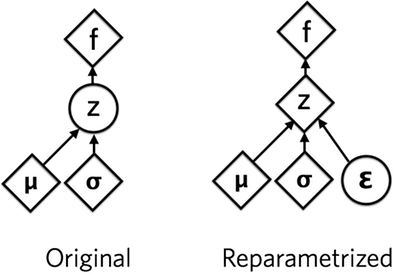
\includegraphics[width=1\textwidth]{reparametrization_trick.png}
        \caption{Minh họa ``Reparametrization trick''. Reparametrization trick giúp ta loại bỏ tính ngẫu nhiên khi lấy mẫu dữ liệu từ phân phối xác suất. Nút hình thoi thể hiện biến cố định, nút hình tròn thể hiện cho biến ngẫu nhiên.}
        \label{fig_repatrick}
    \end{figure}

    ``Reparametrization trick'' là một phương pháp được sử dụng trong mô hình Variational Auto-Encoder để có thể cập nhật trọng số $\phi$ mà $z_u$ vẫn đảm bảo là được lấy mẫu từ phân phối xác suất $q_\phi(z_u|\tilde{x_u})$. 
    Bằng cách ta lấy mẫu $\epsilon \sim \mathcal{N}(0,I_K)$ và khi đó ta tính $z_u$ thông qua công thức:
    \begin{equation}
        z_u = \mu_\phi(\tilde{x}_u) + \epsilon \odot \sigma_\phi(\tilde{x}_u)
    \end{equation}

    theo đó thì $z_u$ thì vẫn là một giá trị được lấy mẫu ngẫu nhiên từ phân phối xác suất trả về từ encoder, nhưng $z_u$ vẫn được tính thông qua phép tính với dấu bằng `='.
    
    Dựa vào ``Reparametrization trick'' ta đã có thể cập nhật trọng số cho mô hình variational Auto-Encoder thông qua thuật toán lan truyền ngược. 
    Hình \ref{fig_repatrick} thể hiện cho ý tưởng của ``Reparametrization trick''.
    \subsubsection{Quá trình đưa ra gợi ý sản phẩm cho người dùng}

    \subsubsection{Lý do ``Variational Auto-Encoder'' phù hợp với bài toán xây dựng hệ thống gợi ý sản phẩm}

    Ly do chúng tôi lựa chọn
    \label{why_vae}
    something in here
    \subsection{Dùng hàm chi phí trong quá trình huấn luyện phù hợp hơn với bài toán gợi ý sản phẩm}


    \subsubsection{``Multinomial likelihood''}
    \label{mulll}
    \begin{figure}
        \centering
        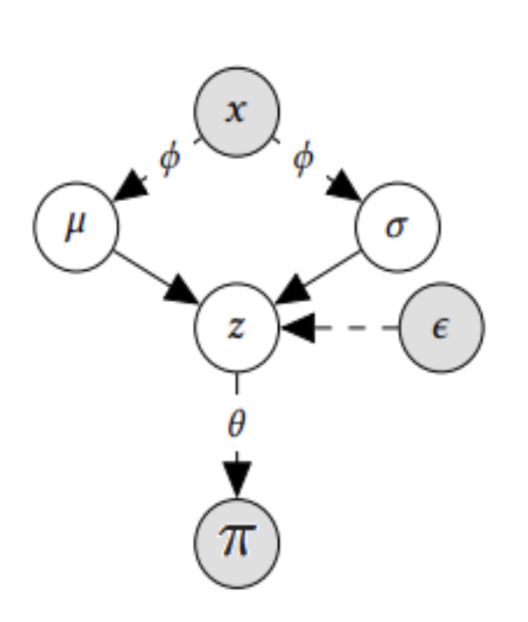
\includegraphics[width=0.5\textwidth]{vae.png}
        \caption{Minh họa kiến trúc mô hình ``Variational Auto-Encoder'' cho bài toán gợi ý sản phẩm}
        \label{fig_mvae}
    \end{figure}
    Trong bất kỳ mô hình học máy nào, hàm lỗi luôn đóng một vai trò cực kỳ quan trọng trong việc quyết định đến độ hiệu quả của mô hình. 
    Hàm lỗi sẽ định nghĩa mục tiêu mà mô hình cần đạt được thông qua việc ước lượng sự khác biệt giữa giá trị được dự đoán của mô hình trả về so giá trị thực tế của nó.
    Ngoài ra, việc tìm được bộ tham số tốt nhất của mô hình cũng dựa cách tìm ra bộ tham số để tối thiểu hàm này.
    Do đó việc lựa chọn một hàm lỗi phù hợp sẽ ảnh hưởng ít nhiều đến kết quả của mô hình 

    Sau khi xác định được hàm lỗi thì ta sẽ có thể dễ dàng sử dụng phương pháp ``Maximum Likelihood Estimation'' như đã được trình bày trong phần \ref{sec_mle}.

<<<<<<< HEAD
    Nhưng khác với Auto-Encoder, hay cả Variational Auto-Encoder thông thường, thì tác giả trong bài báo \cite{mvae} đã giả định rằng 
=======
    Nhưng khác với ``Auto-Encoder'', hay cả ``Variational Auto-Encoder'' thông thường, tác giả trong bài báo \cite{mvae} đã giả định rằng 
>>>>>>> 1fb170123ba595a507b570a6bb9f69e8c4a0167d
    \begin{equation}
        \label{asumpt_xu}
        x \sim \text{Mul}(N_u,\pi({z_u}))
    \end{equation}
<<<<<<< HEAD
    có nghĩa rằng, $x_u$ sẽ được phát sinh từ một phân phối xác suất, cụ thể là phân phối đa thức (multinomial).
=======
    có nghĩa rằng, $x_u$ sẽ được phát sinh từ một phân phối xác suất, cụ thể là phân phối đa thức (``Multinomial Distribution'').
>>>>>>> 1fb170123ba595a507b570a6bb9f69e8c4a0167d
    Với $\pi(z_u)$ là một véc-tơ xác suất thể hiện cho xác suất được chọn của tập $N_u$ sản phẩm  với $N_u$ là số lượng sản phẩm mà người dùng $u$ đẫ tương tác. 
    Ta gọi $f_\theta(z_u) \equiv [f_{u1}, f_{u2}, \dots , f_{uI}] $ 
    là kết quả trả về từ decoder, với đầu vào là đặc trưng ẩn $z_u$.
    Theo đó $\pi(z_u)$ được tính như sau:
    \begin{equation}
        \label{mult-ll}
        \pi(z_u)_{ui} = \frac{\exp(f_{ui})}{\sum_j(\exp(f_{uj}))}
    \end{equation}
    trong đó, $u\in \mathcal{U}$ và $i \in \mathcal{I}$.
    
    
    Với giả định này thì ở mạng decoder, sau khi nhận đầu vào $z_u$ sẽ trả về véc-tơ $\pi(z_u)$ trên toàn bộ tập sản phẩm trong hệ thống. 
    Hình \ref{fig_mvae} thể hiện kiến trúc mà tác giả đã sử dụng. 
    Theo đó hàm lỗi được tác giả sử dụng trong trường hợp bài toán xây dựng hệ thống gợi ý sản phẩm là ``Multinomial log likelihood'' 
    \begin{equation}
        \log p_\theta(x_u|z_u) = \sum_i x_{ui}\log (\pi_i(z_u))
    \end{equation}
<<<<<<< HEAD
    
    Hàm lỗi này thì thường được sử dụng trong những mô hình ngôn ngữ như latent Dirichlet allocation, và kinh tế multinomial logit choice model. 
    Multinomial likelihood thường được sử dụng với những bài toán liên quan đến dữ liệu chuỗi thời gian (time-series) hay dữ liệu dạng chuỗi (sequence) tuy nhiên lại ít được tập trung, nghiên cứu sử dụng trong lĩnh vực mô hình đặc trưng ẩn. 
=======
    Hàm lỗi này thì thường được sử dụng trong những mô hình ngôn ngữ như ``Latent Dirichlet allocation'', và kinh tế ``Multinomial logit choice model''. 
    ``Multinomial likelihood'' thường được sử dụng với những bài toán liên quan đến dữ liệu chuỗi thời gian (time-series) hay dữ liệu dạng chuỗi (sequence) tuy nhiên lại ít được tập trung, nghiên cứu sử dụng trong lĩnh vực mô hình đặc trưng ẩn. 
>>>>>>> 1fb170123ba595a507b570a6bb9f69e8c4a0167d
    Ở mô hình này, thì tác giả trong bài báo \cite{mvae} đã sử dụng hàm lỗi này cho bài toán gợi ý sản phẩm dựa trên giả định \ref{asumpt_xu}.
    Lý do mà tác giả đã sử dụng hàm này bởi vì 
    ``Multinomial log-likelihood'' sẽ đặt giá trị thể hiện độ lớn xác suất lên tập sản phẩm được gợi ý mà mô hình trả về. 
    Vì tổng độ lớn xác suất sẽ phải bằng 1, do đó các sản phẩm được mô hình gợi ý sẽ phải ``cạnh tranh'' với nhau để có được giá trị xác suất cao hơn. 
    Do đó, mô hình sẽ cố gắng đạt được mục tiêu là các sản phẩm trả về sẽ được xếp hạng đúng theo mức độ phù hợp với người dùng. 
    
    \subsubsection{Một góc nhìn khác của hàm ELBO}
    \label{subsubsecELBO}
    Theo hàm mục tiêu được định nghĩa ở công thức \ref{elbo_mvae}, ở một góc nhìn khác ta có thể phân tích 2 thành phần cấu thành ELBO với 2 mục tiêu khác nhau.
    Ở thành phần đầu tiên, sẽ thể hiện cho độ lỗi tái tạo lại tương tác của người dùng, hay là tập sản phẩm được gợi ý có đúng với nhu cầu người dùng hay không. 
    Thành phần thứ hai, thì ta có thể xem như là một ``regularization'' cho hàm lỗi.
    Góc nhìn này, ta đã được thảo luận qua ở mục \ref{trade_off} thì đây cũng chính là việc đánh đổi giữa độ lỗi trong việc mô hình hóa dữ liệu và chuẩn hóa cho đặc trưng ẩn gần với phân phối chuẩn trong mô hình variational Auto-Encoder.

    Với một bài toán phát sinh dữ liệu mới, thì đánh đổi này là cần thiết bởi nó sẽ đảm bảo cho dữ liệu mới được phát sinh được chuẩn hóa.
    Nhưng trong bài gợi ý sản phẩm thì ta quan tâm hơn việc mô hình hóa dữ liệu hơn là việc đảm bảo các tính chất xác suất của đặc trưng ẩn.
    Do đó tác giả đã đề xuất sử dụng một siêu tham số $\beta$ để có thể dễ dàng kiểm soát được đánh đổi đã được nói ở trên. 
    Siêu tham số là một hệ số không được học từ mô hình mà được chỉ định trước cho mô hình để có thể huấn luyện.
    Theo đó, hàm mục tiêu lúc này của mô hình sẽ là:
    \begin{equation}
        \label{elbo_betamvae}
        \mathcal{L}(x_u;\phi,\theta) = E_{q_\phi(z_u|x_u)}[\log p_\theta(x_u|z_u)] - \beta \times \mathbb{KL}(q_\phi(z_u|x_u) || p(z_u))
    \end{equation}

    Với đề xuất này, thì việc huấn luyện mô hình sẽ phải bao gồm thêm việc lựa chọn siêu tham số cho mô hình.
    Trong nhiều trường hợp thì việc lựa chọn siêu tham số là một bước mà tốn kém thời gian khi ta phải đánh giá mô hình trên nhiều giá trị siêu tham số khác nhau.  
    Do đó tác giả cũng đề xuất thêm một phương pháp được gọi là ``KL-annealing''.
    Phương pháp này là một phương pháp ``heuristic'' để lựa chọn siêu tham số cho mô hình.
    Ý tưởng của phương pháp là ban đầu ta sẽ gán giá trị cho $\beta =0$.
    Và beta được tăng dần giá trị $\beta$ cho đến một giá trị cố định nào đó sau mỗi lần cập nhật trọng số của mô hình.
    Ở bài báo \cite{mvae} thì tác giả tăng dần $\beta$ từ 0 cho đến 1 thì dừng cập nhật cho $\beta$.

    Khi huấn luyện mô hình với phương pháp này thì sau mỗi lần cập nhật mô hình thì ta sẽ đánh giá lại mô hình và lưu lại giá trị $\beta$ sau mỗi lần mà mô hình đạt kết quả tốt hơn trên tập kiểm định.
    Tiếp theo đó thì để mô hình có thể đạt được một kết quả tốt hơn thì ta sẽ thực hiện huấn luyện lại mô hình một lần nữa với giá trị $\beta$ tốt nhất đã được lưu lại trước đó.  Ngoài ra, nếu chi phí tài nguyên không cho phép, ta chỉ có thể huấn luyện mô hình chỉ trong một lần thì ta có thể dừng cập nhật lại giá trị $\beta$ sau khi mô hình có dấu hiệu giảm độ hiệu quả trên tập kiểm định. 
